\documentclass[11pt,a4paper,oneside]{article}
\usepackage[latin1]{inputenc}
\usepackage{amsmath}
\usepackage{amsfonts}
\usepackage{amssymb}
\usepackage{graphicx}
\usepackage{color}
\usepackage {tikz}
\usepackage{fancyvrb}
\usetikzlibrary {er}
\usepackage[left=2.00cm, right=2.00cm, top=1.00cm]{geometry}
\graphicspath{{./}}
\fvset{tabsize=4}

\begin{document}
	\title{DS 255 - System Virtualization \\ Assignment III - Constructs and Mechanisms for Virtualization}
	\author{Shriram R. \\ M Tech (CDS) \\ 06-02-01-10-51-18-1-15763}
	\maketitle	
	
	\begin{enumerate}
		\item
		\item
		\item Virtualization is not exactly the same as abstraction but somewhat similar. Virtualization differs in the sense that it does not necessarily hide details (i.e) the level of detail in a virtual system is often same as that of the real system. While the goal of abstraction is to hide the complexities of one layer in a system from another. However, both virtualization and abstraction provides an additional layer of interface between two existing layers in a system.
		
	    Example: An hard disk is divided into sectors, tracks etc. But an application can read/write files in hard disk without the knowledge of structure of hard disk. This is abstraction where details are hidden. A Virtual machine can perform all kind of operations that it would perform on a real hardware. This is virtualization where the same level of interface / details is available to virtual machine. 
		
		\item \textbf{ISA} - Instruction Set Architecture (ISA) is the interface between hardware and software layer of a system. Application programs and operating system code interact with the hardware through ISA. It is generally divided into user and system ISAs targeted for user applications and OS operations respectively. All System VMs are defined in this layer.
		
		\textbf{ABI} - Application Binary Interface (ABI) provides applications with user instructions (user ISA) and system call interface. The system call interface is used to request privileged functions related to shared hardware etc. Note that the system ISA is not exposed to applications in this interface. Process VMs are defined in this layer.
		
		\textbf{API} - Application Programming Interface (API) provides access to user ISA and standard libraries. Applications can invoke various system services through the library. The API provides an abstraction (sometimes a wrapper) to the implementation of these services. High Level Language (HLL) VMs are defined in this layer. 
		\item 
		\item
		\item  
		\item Desirable characteristics in an ISA for Emulation are as follows,
		      \begin{enumerate}
		      	\item Self-modifying and self-referencing code should not be permitted as it incurs additional challenges and overhead to emulation
		      	\item Stack oriented memory architecture with an abstract memory model if infinite size is desirable as it allows for simple maintenance of program state
		      	\item Indirect jumps should not be permitted as it will cause additional overhead to emulation in terms of finding the code location
		      	\item Precise exception state requirement has to be relaxed and traps should be limited. This means that the exceptions are tested within the program
		      	\item Variable length instructions, padding and mixing of code and data should not be permitted as it poses challenges in code discovery	      	
		      \end{enumerate}
		    
	         %\begin{center}
	         %   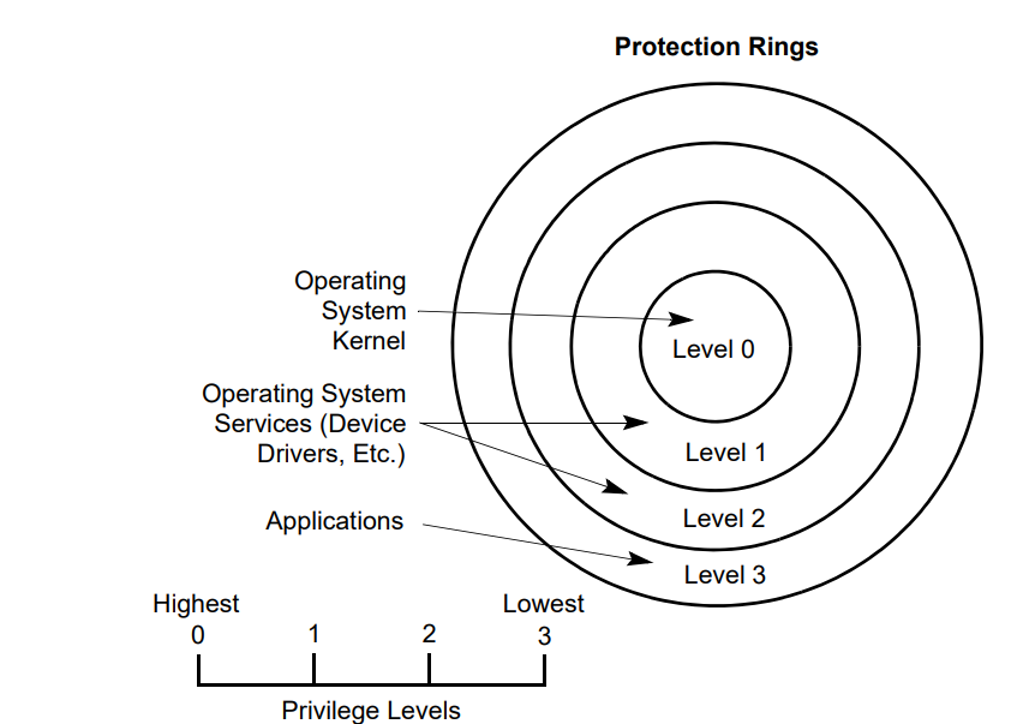
\includegraphics[scale=0.6]{1.png}	[4]
	         %\end{center}			
	\end{enumerate}
    
    \textbf{References}
    \begin{enumerate}
    	\item To be Added    	
    \end{enumerate}
 

    
\end{document}